\chapter{Środowisko symulacyjne}
\label{cha:rozdzial4}

Gdy projektowano pierwsze maszyny, które miały wykonywać konkretne zadania, opierano
się na dokładnych modelach matematycznych opisujących fizykę. Nie istniały narzędzia
do weryfikacji skuteczności działania danego urządzenia. Dopiero rozwój technologii
komputerowych i wzrost mocy obliczeniowej procesorów umożliwił bardzo szybką 
weryfikację stworzonych maszyn na komputerach, które w kilka sekund były w stanie 
sprawdzić poprawność obliczeń. Duże znaczenie symulacje zaczęły odgrywać kiedy
testowanie projektowanych maszyn mogło sprawiać zagrożenia dla ludzi czy samego
środowiska, w którym były testowane.

Ze względu na coraz niższą cenę sprzętu komputerowego i rozwojowi oprogramowania,
coraz więcej osób może w swoich domach uruchamiać modele wielu urządzeń bez ryzyka
uszkodzenia czegokolwiek i móc prowadzić swoje badania. W poniższej pracy konieczne
było zastosowanie takiego środowiska symulacyjnego, ponieważ testowane rozwiązania
są nowe i agenci uczenia motywowanego mogą czasem wykonywać czynności, które nie
były uwzględnione przez projektanta, zgodnie z tabelą \ref{tab:ml_vs_rl}.

W poniżej pracy uczenie motywowane będzie testowane na robocie mobilnym w środowisku
symulacyjnym Gazebo Sim \cite{gazebo_sim_website}.

\section{Symulator Gazebo}

Rozwój symulatora Gazebo rozpoczął się jesienią 2002 roku na Uniwersytecie 
Południowej Kalifornii. Oryginalnymi twórcami byli dr Andrew Howard i jego 
uczeń Nate Koenig. Koncepcja symulatora o wysokiej wierności wynikała z potrzeby 
symulacji robotów w środowiskach zewnętrznych w różnych warunkach. 
Jako komplementarny symulator do Stage, nazwa Gazebo została wybrana jako 
struktura najbliższa scenie zewnętrznej. Nazwa utknęła pomimo faktu, że 
większość użytkowników Gazebo symuluje środowisko wewnętrzne.

Symulator ten ma zintegrowane silnik fizyki ODE (Open Dynamics Engine). Wykorzystuje
renderowanie korzystając z OpenGL. Dzięki temu możeliwe jest symulowanie wielu 
rodzajów sensorów:

\begin{itemize}
    \item ciśnieniomierz,
    \item wysokościomierz,
    \item kamera (RGB, głębi),
    \item czujnik kontaktu (dotyku),
    \item czujnik nacisku,
    \item GPS,
    \item lidar,
    \item skaner laserowy,
    \item IMU (ang. \textit{inertial measurement unit}),
    \item magnetometr,
    \item czujnik odległości,
    \item inne.
\end{itemize}

Tak duży zasób czujników umożliwia sprawdzanie na wiele sposobów jaki zestaw 
sensorów może być wykorzystany dla konkretnych celów oraz sprawia, że testowanie
nowych funkcjonalności bez ryzyka uszkodzenia robota czy środowiska. 

Graficzny interfejs umożliwia szybkie projektowanie nowych robotów czy elementów
środowiska. Wygląd głównego okna, w którym wykonywana jest większość pracy
podczas projektowania środowiska symulacyjnego pokazano na rysunku 
\ref{fig:gazebo_main_window}.

\begin{figure}[h]
    \centering
    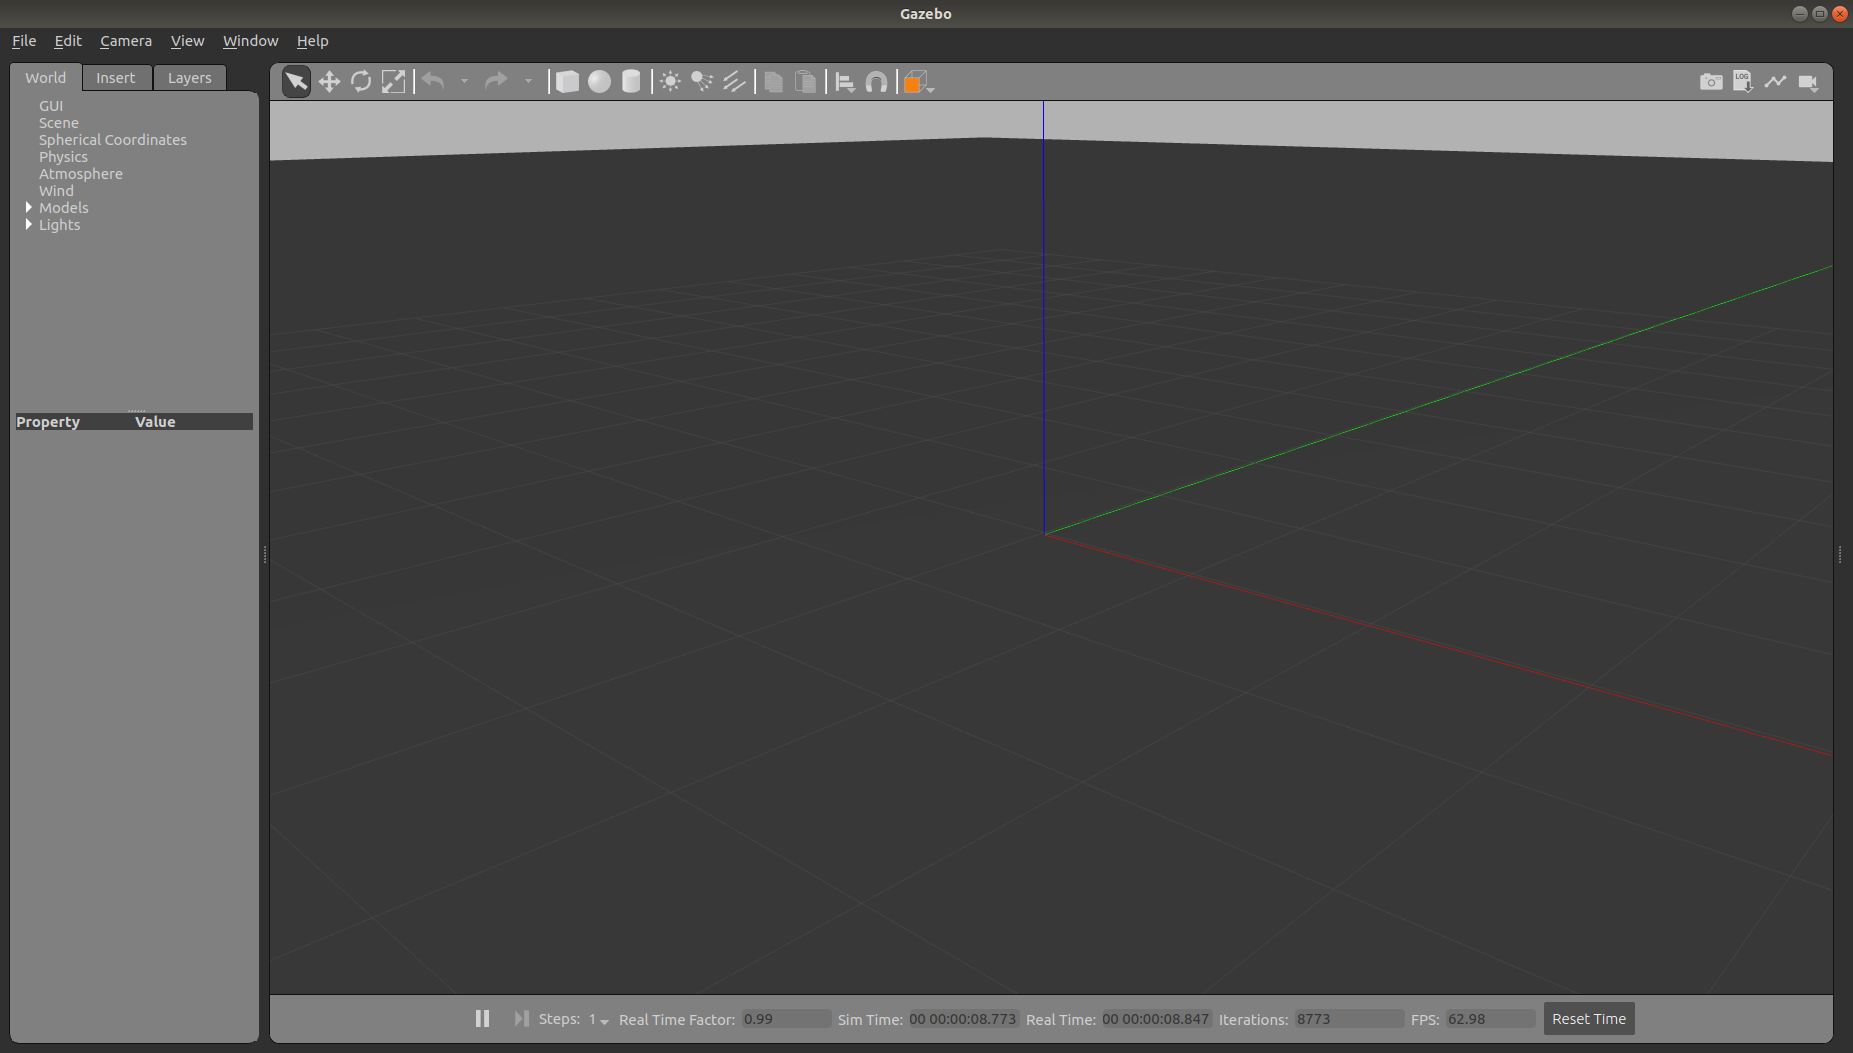
\includegraphics[width=0.7\linewidth]{rozdzial5/images/gazebo_main_window}
    \caption{Główne okna symulatora Gazebo. Źródło: opracowanie własne.}
    \label{fig:gazebo_main_window}
\end{figure}

Dodatkowowo w Gazebo oprócz silnika fizycznego ODE można skorzystać także z innych
bardzo popularnych silników fizyczny jak: Bullet. Dzięki rzeczywistemu renderowaniu
sceny w kamerach możliwe jest testowanie systemów wizyjnych. Takie na pewno
muszą być zastosowane dla agenta z uczeniem motywowanym, ponieważ to jeden
z podstawowych sensorów stosowanych przez człowieka na etapie poznawania nowego
środowiska.

Środowisko Gazebo Sim składa się z kilku elementów, które sprawiają, że możliwe
jest uruchomienie symulacji robota. Są to zgodnie z \cite{gazebo_components}.

